\section{Redes Neuronales}

%%%%%%%%%%%%%%%%%%%%%%%%%%%%%%%%%%%%%%%%%%%%%%%%%%%%%%%%%%%%%%%%%%%%%%%%%%%%%%%%%%%%
%%%%%%%%%%%%%%%%%%%%%%%%%%%%%%%%%%%%%%%%%%%%%%%%%%%%%%%%%%%%%%%%%%%%%%%%%%%%%%%%%%%%
%%%%%%%%%%%%%%%%%%%%%%%%%%%%%%%%%%%%%%%%%%%%%%%%%%%%%%%%%%%%%%%%%%%%%%%%%%%%%%%%%%%%

\subsection{Redes Neuronales Prealimenadas}

%%%%%%%%%%%%%%%%%%%%%%%%%%%%%%%%%%%%%%%%%%%%%%%%%%%%%%%%%%%%%%%%%%%%%%%%%%%%%%%%%%%%%



\begin{frame}


    \begin{figure}
        \hspace*{-1cm}   
        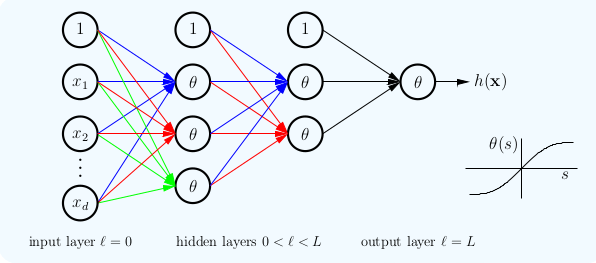
\includegraphics[keepaspectratio=true,height=1\paperheight,width=0.99\linewidth]{Images/grafo RRNN.png}
    \end{figure}
    
    Entrenamiento: 
    \begin{itemize}
        \item Optimización $\rightarrow$ Método del Gradiente Descendiente
        \item Cálculo del gradiente $\rightarrow$ Algoritmo BackPropagation
    \end{itemize}

\end{frame}


%%%%%%%%%%%%%%%%%%%%%%%%%%%%%%%%%%%%%%%%%%%%%%%%%%%%%%%%%%%%%%%%%%%%%%%%%%%%%%%%%%%%
%%%%%%%%%%%%%%%%%%%%%%%%%%%%%%%%%%%%%%%%%%%%%%%%%%%%%%%%%%%%%%%%%%%%%%%%%%%%%%%%%%%%
%%%%%%%%%%%%%%%%%%%%%%%%%%%%%%%%%%%%%%%%%%%%%%%%%%%%%%%%%%%%%%%%%%%%%%%%%%%%%%%%%%%%

\subsection{Redes Neuronales Convolucionales}


%\begin{frame}{Operación de Convolución - Señales}
%
%    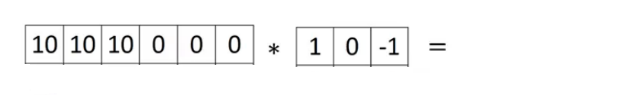
\includegraphics[scale=0.5]{Images/convolution5 (2).png}
%    \pause
%    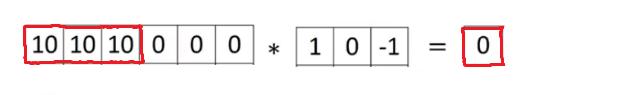
\includegraphics[scale=0.5]{Images/convolution (2).png}
%    \pause
%    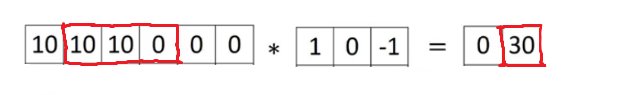
\includegraphics[scale=0.5]{Images/convolution2 (2).png}
%    \pause
%    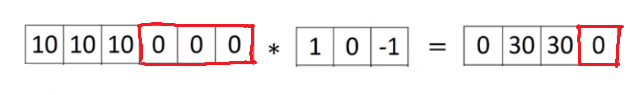
\includegraphics[]{Images/convolution4.png}
%    \pause
%    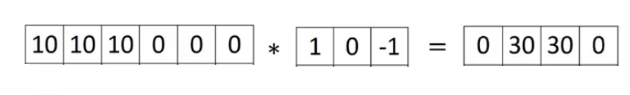
\includegraphics[]{Images/convolution5.png}
%    
%\end{frame}

%%%%%%%%%%%%%%%%%%%%%%%%%%%%%%%%%%%%%%%%%%%%%%%%%%%%%%%%%%%%%%%%%%%%%%%%%%%%%%%%%%%%%

%\begin{frame}{Operación de Convolución - Imágenes}
%
%    \begin{columns}
%        \column{0.6\textwidth}\centering
%            \begin{figure}
%            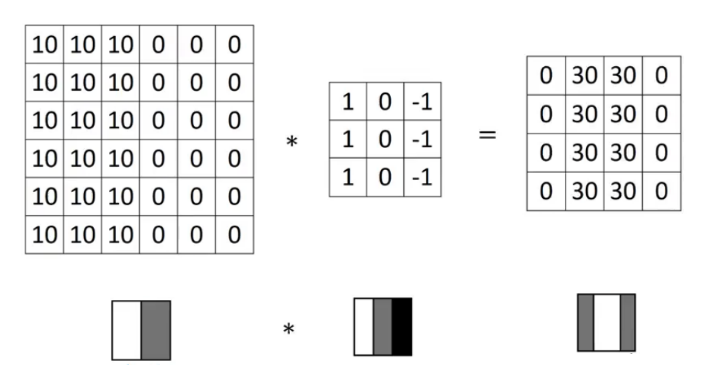
\includegraphics[width=1\linewidth]{Images/convolution operation.png}
%            \end{figure}
%            
%                
%            Parámetros de la convolución:
%                \begin{itemize}
%                    \item Zancada (Stride)
%                    \item Dilatación
%                    \item Tamaño del kernel
%                    \item Padding
%                \end{itemize}
%
%        \column{0.5\textwidth}\centering
%            \begin{figure}
%            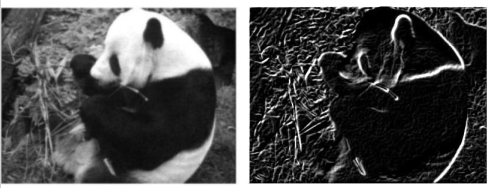
\includegraphics[width=1\linewidth]{Images/ejemplo_conv2.png}
%            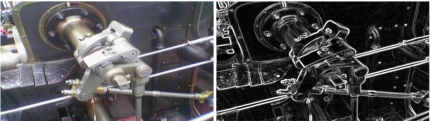
\includegraphics[width=1\linewidth]{Images/ejemplo_conv3.png}
%            \end{figure}
%    \end{columns}
%    
%\end{frame}


%%%%%%%%%%%%%%%%%%%%%%%%%%%%%%%%%%%%%%%%%%%%%%%%%%%%%%%%%%%%%%%%%%%%%%%%%%%%%%%%%%%%%

\begin{frame}{Idea General de una CNN}

    \begin{figure}
            \hspace*{-1cm}   
            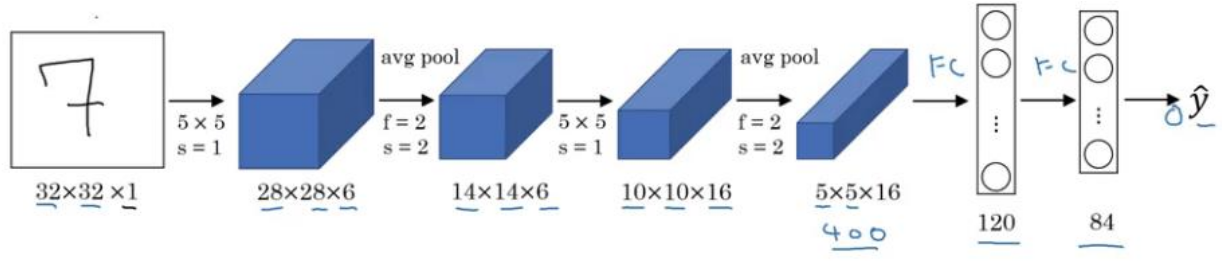
\includegraphics[keepaspectratio=true,height=1\paperheight,width=0.99\paperwidth]{Images/idea of cnn.png}
    \end{figure}
    \pause
    \begin{columns}
        \column{0.6\textwidth}\centering
        Capas de una CNN
        \begin{itemize}
            \item Capas de convolución
            \item Capas de pooling 
            \item Capas de normalización
            \item Capas totalmente conectadas.
        \end{itemize}
    \pause
        \column{0.5\textwidth}\centering
        \begin{figure}
            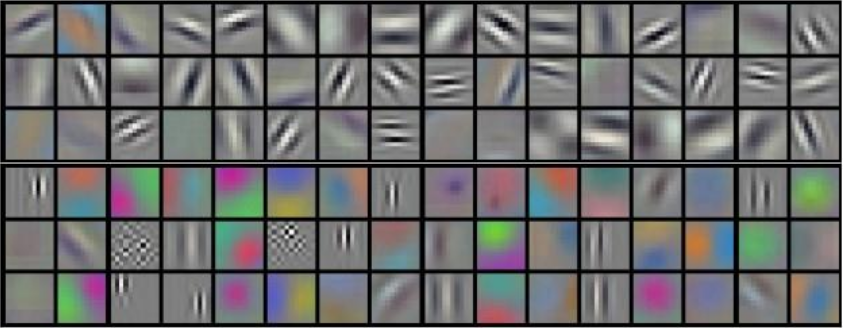
\includegraphics[width=1\linewidth]{Images/filtrosAlexNet.png}
            \caption{Ejemplos de filtros aprendidos por el modelo AlexNet en su primera capa. (ImageNet2012)}
        \end{figure}
    \end{columns}
\end{frame}


%\begin{frame}{Idea General de una CNN}
%
%    \begin{figure}
%            \hspace*{-1cm}   
%            \includegraphics[keepaspectratio=true,height=1\paperheight,width=1\paperwidth]{Images/id%ea of cnn 2.png}
%    \end{figure}
%
%\end{frame}



%%%%%%%%%%%%%%%%%%%%%%%%%%%%%%%%%%%%%%%%%%%%%%%%%%%%%%%%%%%%%%%%%%%%%%%%%%%%%%%%%%%%
%%%%%%%%%%%%%%%%%%%%%%%%%%%%%%%%%%%%%%%%%%%%%%%%%%%%%%%%%%%%%%%%%%%%%%%%%%%%%%%%%%%%
%%%%%%%%%%%%%%%%%%%%%%%%%%%%%%%%%%%%%%%%%%%%%%%%%%%%%%%%%%%%%%%%%%%%%%%%%%%%%%%%%%%%

\subsection{Redes Neuronales Recurrentes}

\begin{frame}{Neurona Recurrente}
    \begin{figure}
        \centering
        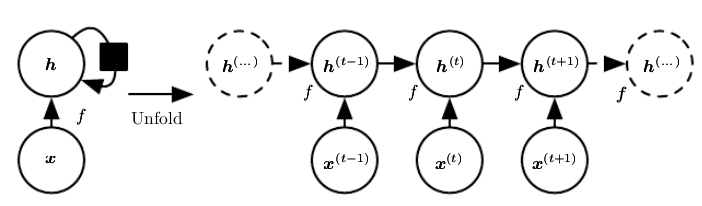
\includegraphics[keepaspectratio=true,height=1\paperheight,width=0.8\paperwidth]{Images/grafo computacional 1.png}
    \end{figure}
\end{frame}

%%%%%%%%%%%%%%%%%%%%%%%%%%%%%%%%%%%%%%%%%%%%%%%%%%%%%%%%%%%%%%%%%%%%%%%%%%%%%%%%%%%%

\begin{frame}{Arquitectura típica de RNN}

    \begin{columns}
        \column{0.5\textwidth}\centering
        \begin{figure}
            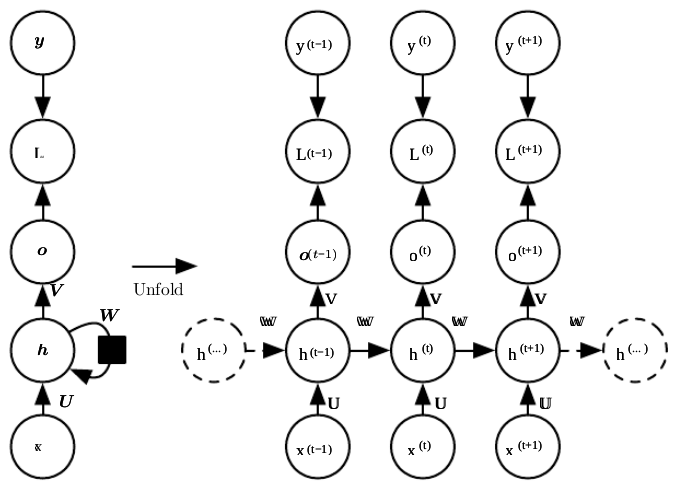
\includegraphics[width=1\linewidth]{Images/grafo 2.png}
        \end{figure}
        
        
        \column{0.5\textwidth}\centering
        \begin{figure}
            \centering
            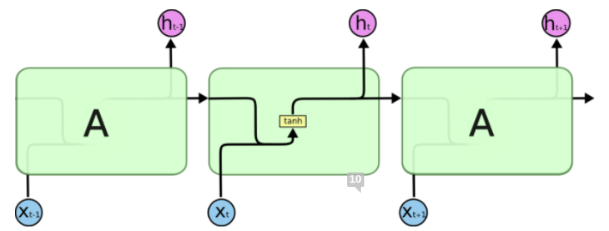
\includegraphics[width=1\linewidth]{Images/rnng.png}
        \end{figure}
        \begin{align*}
                a^{(t)} &= b + Wh^{(t-1)} + Ux^{(t)},\\
                h^{(t)} &= \tanh{(a^{(t)})}, \\
                o^{(t)} &= c + Vh^{(t)}, \\
                \hat{y}^{(t)} &= softmax(o^{(t)})
            \end{align*}
    \end{columns}
    
    
    
\end{frame}

%%%%%%%%%%%%%%%%%%%%%%%%%%%%%%%%%%%%%%%%%%%%%%%%%%%%%%%%%%%%%%%%%%%%%%%%%%%%%%%%%%%%

\begin{frame}{Otras arquitecturas}

    \begin{columns}
        \column{0.5\textwidth}\centering
        \begin{figure}
            \centering
            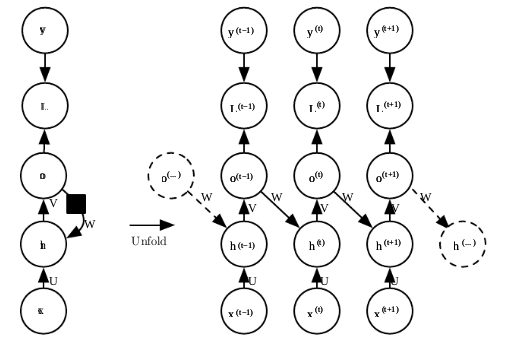
\includegraphics[width=1\linewidth]{Images/rnn tipo.png}
        \end{figure}
    
    
        \column{0.5\textwidth}\centering
        \begin{figure}
            \centering
            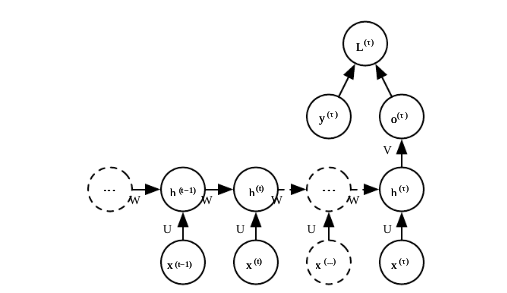
\includegraphics[width=1\linewidth]{Images/rnn tercer tipo.png}
        
        \end{figure}
    \end{columns}
\end{frame}


%%%%%%%%%%%%%%%%%%%%%%%%%%%%%%%%%%%%%%%%%%%%%%%%%%%%%%%%%%%%%%%%%%%%%%%%%%%%%%%%%%%%

\begin{frame}{Long Short Term Memory (LSTM)}
\begin{overprint}
    
    \onslide<1>
    
    \begin{figure}
            \centering
            \vspace{1cm}
            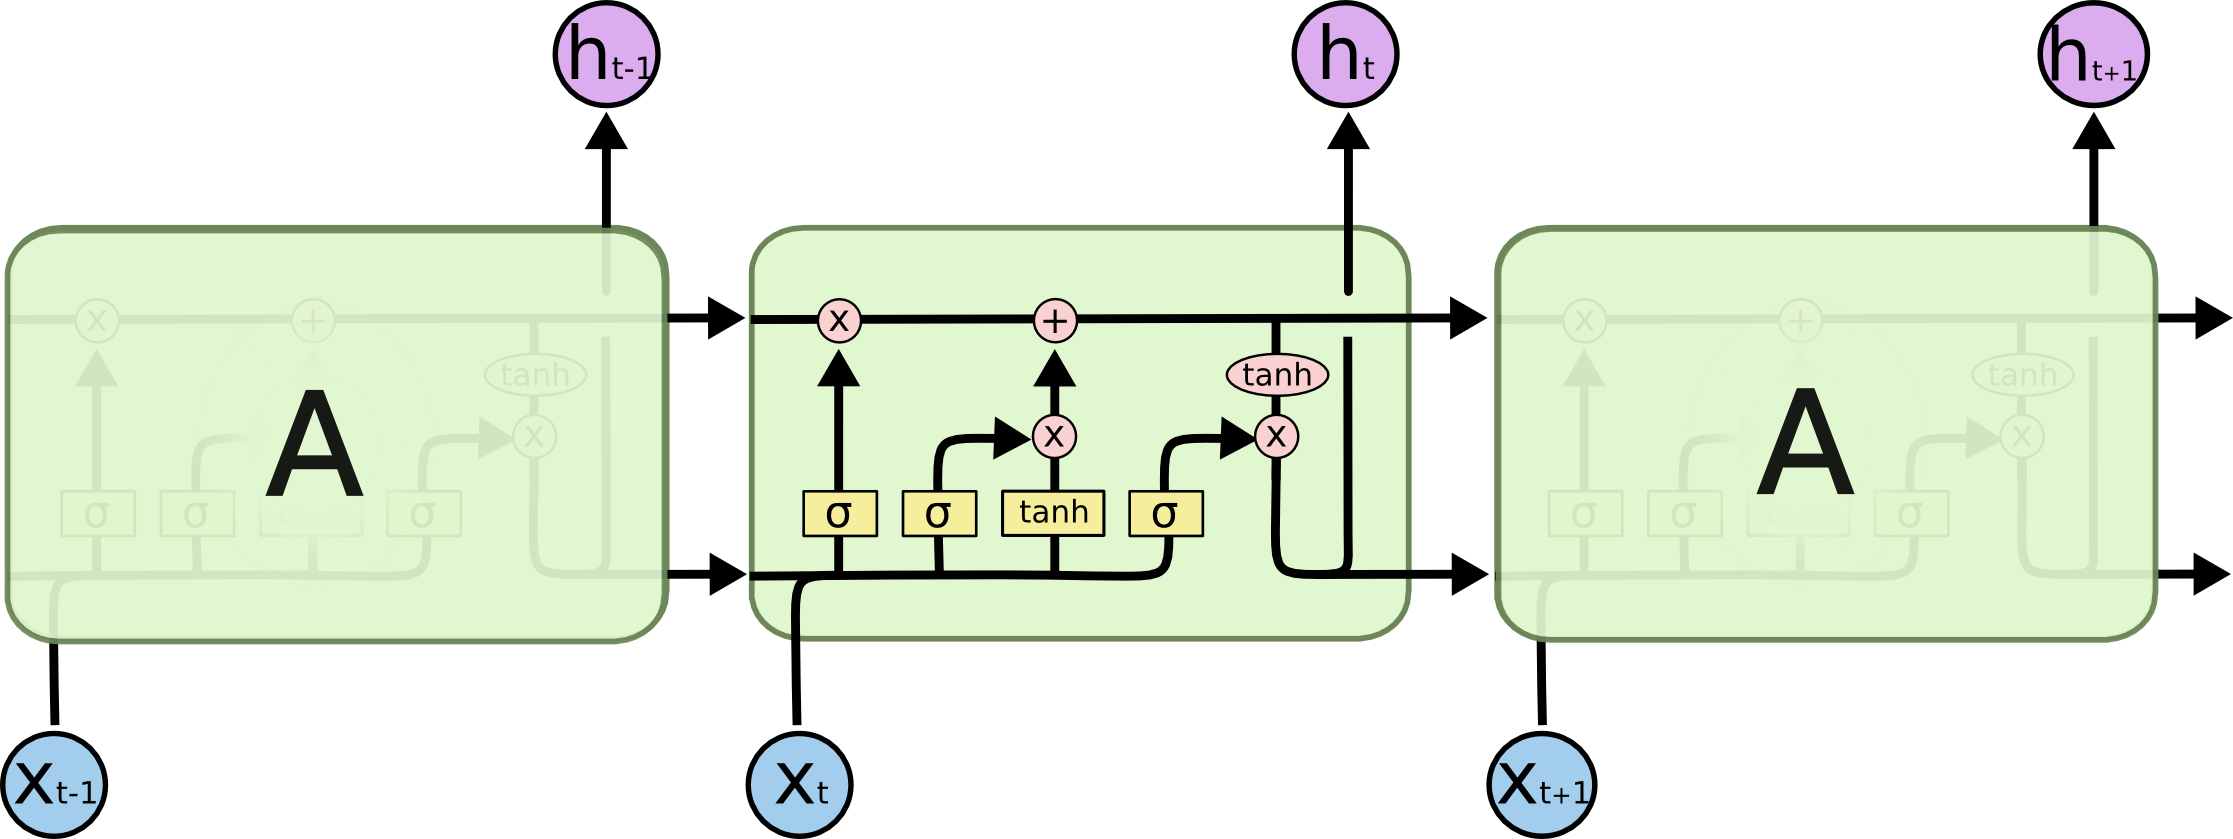
\includegraphics[keepaspectratio=true,height=1\paperheight,width=1\linewidth]{Images/lstmg.png}
        \end{figure}
    \onslide<2>
        \begin{center} \textbf{Estado de la celda} \end{center}
        \begin{figure}
            \centering
            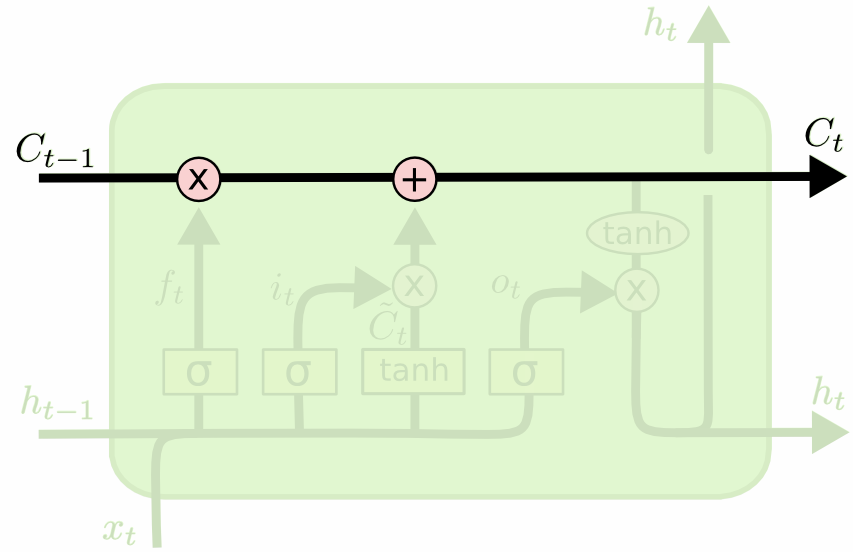
\includegraphics[keepaspectratio=true,height=0.7\paperheight,width=0.7\linewidth]{Images/estado.png}
        \end{figure}

    \onslide<3>
        \begin{center} \textbf{Puerta de Olvido} \end{center}
        \begin{figure}
            \centering
            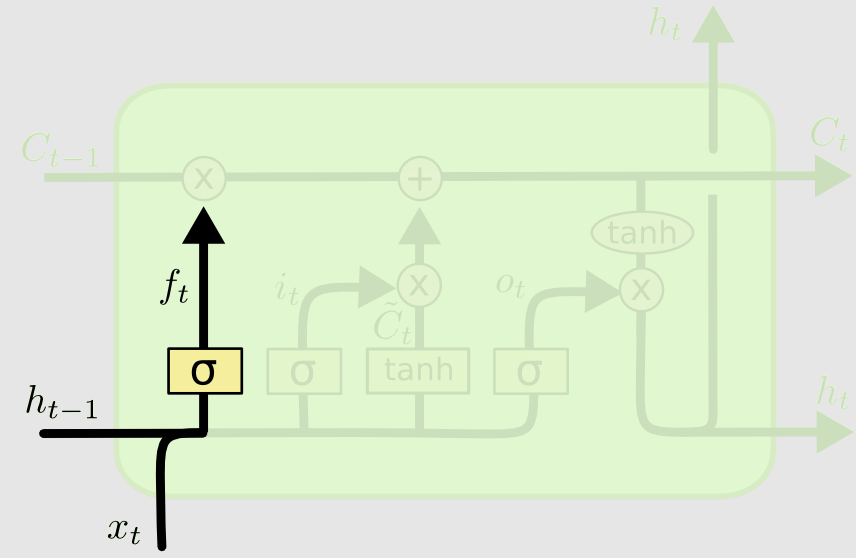
\includegraphics[keepaspectratio=true,height=0.7\paperheight,width=0.7\linewidth]{Images/puerta1.png}
        \end{figure}
        \begin{equation*}
            f^{(t)}_i = \sigma \Big( b^f_i + \sum_j U_{i,j}^f x^{(t)}_j + \sum_j W_{i,j}^f h^{(t-1)}_j \Big) 
        \end{equation*}

    \onslide<4>
        \begin{center} \textbf{Puerta de entrada} \end{center}
        \begin{figure}
            \centering
            \vspace{-0.5cm}
            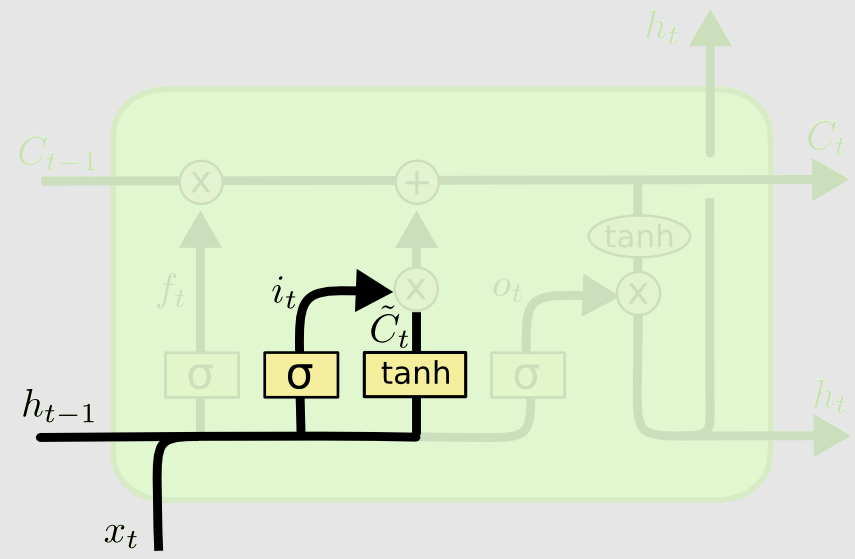
\includegraphics[keepaspectratio=true,height=0.45\paperheight,width=0.7\linewidth]{Images/puerta2.png}
        \end{figure}
        \begin{equation*}
            \begin{aligned}
                g^{(t)}_i & = \sigma \Big( b^g_i + \sum_j U_{i,j}^g x^{(t)}_j + \sum_j W_{i,j}^g h^{(t-1)}_j \Big) \\
                \tilde{C}^{(t)} & = \tanh \Big( b^C_i + \sum_j U^C_{i,j}x^{(t)}_j + \sum_j W^C_{i,j} h^{(t-1)}_j \Big)
            \end{aligned}
        \end{equation*}
       
    \onslide<5>
        \begin{center} \textbf{Actualizació}n \end{center}
        \begin{figure}
            \centering
            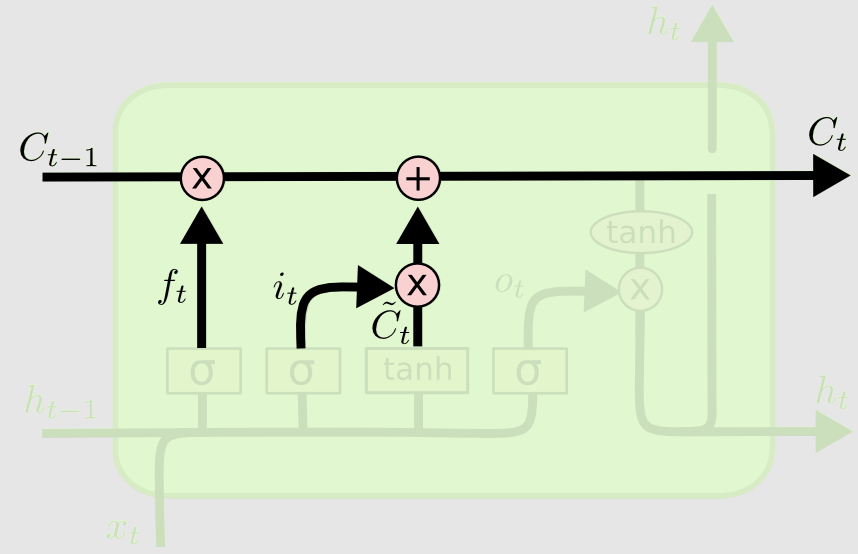
\includegraphics[keepaspectratio=true,height=0.7\paperheight,width=0.7\linewidth]{Images/puerta3.png}
        \end{figure}
        \begin{equation*}
        C^{(t)}_i = f^{(t)}_i * C^{(t-1)}_i + g^{(t)}_i * \tilde{C}_i^{(t)}
        \end{equation*}
    \onslide<6>
        \begin{center} \textbf{Puerta de salida} \end{center}
        \begin{figure}
            \centering
            \vspace{-0.5cm}
            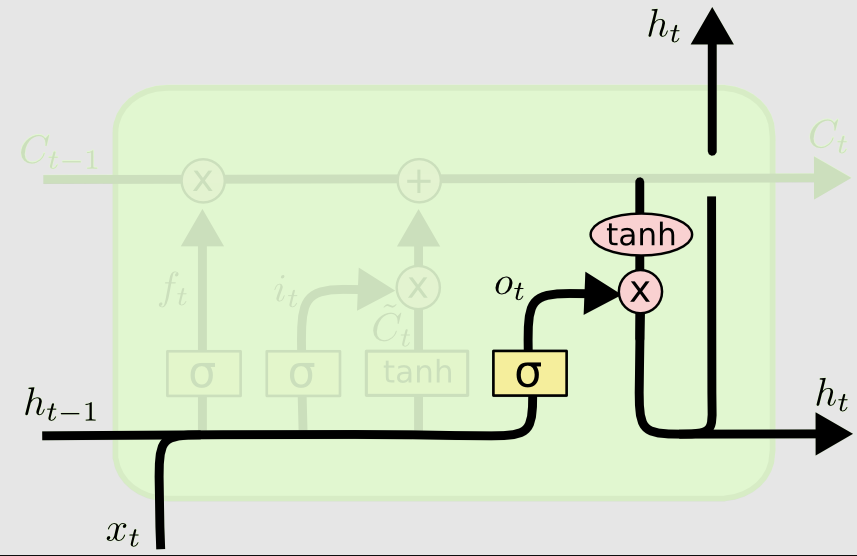
\includegraphics[keepaspectratio=true,height=0.6\paperheight,width=0.65\linewidth]{Images/puerta4.png}
        \end{figure}
        \begin{equation*}
            \begin{aligned}
                o^{(t)}_i & = \sigma \Big( b^o_i + \sum_j U^o_{i,j} x^{(t)}_j + \sum_j W^o_{i,j} h^{(t-1)}_j \Big) \\
                h^{(t)}_i & = tanh \big( C^{(t)}_i \big) * o^{(t)}_i
            \end{aligned}
        \end{equation*}
        
       
\end{overprint}
\end{frame} 


%%%%%%%%%%%%%%%%%%%%%%%%%%%%%%%%%%%%%%%%%%%%%%%%%%%%%%%%%%%%%%%%%%%%%%%%%%%%%%%%%%%%
\begin{frame}{Variaciones LSTM}

    \begin{columns}
        \column{0.5\textwidth}\centering
        \begin{figure}
            \centering
            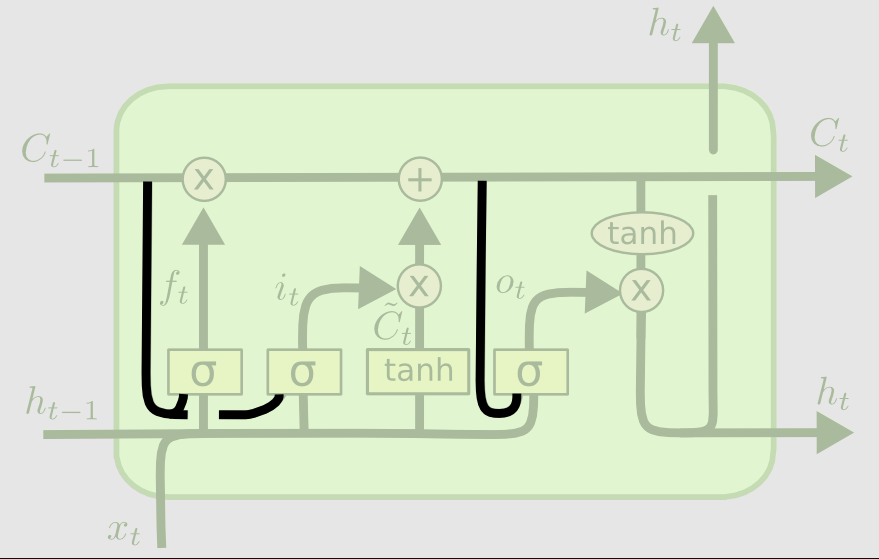
\includegraphics[width=1\linewidth]{Images/var1.png}
        \end{figure}
    
    
        \column{0.5\textwidth}\centering
        \begin{figure}
            \centering
            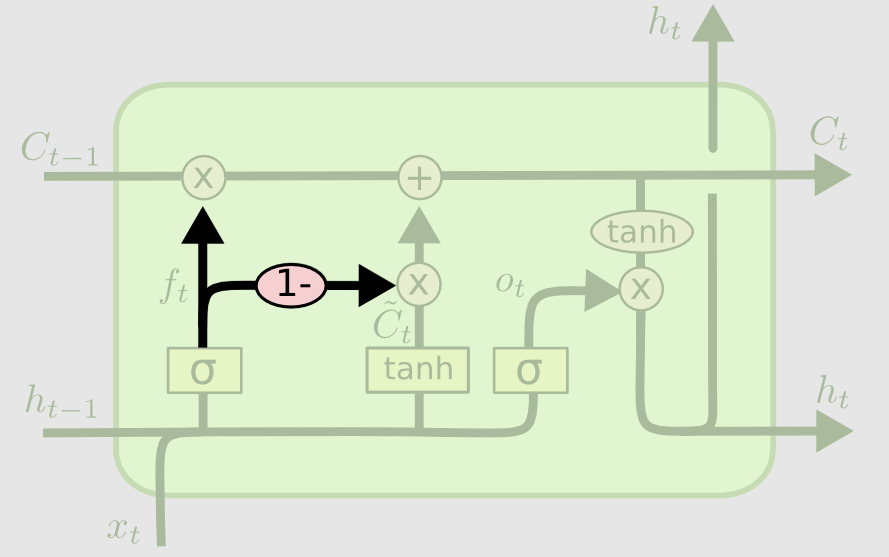
\includegraphics[width=1\linewidth]{Images/var2.png}
        
        \end{figure}
    \end{columns}
    
\end{frame}

%%%%%%%%%%%%%%%%%%%%%%%%%%%%%%%%%%%%%%%%%%%%%%%%%%%%%%%%%%%%%%%%%%%%%%%%%%%%%%%%%%%%
\begin{frame}{Gated Recurrent Unit (GRU)}

\begin{figure}
    \centering
    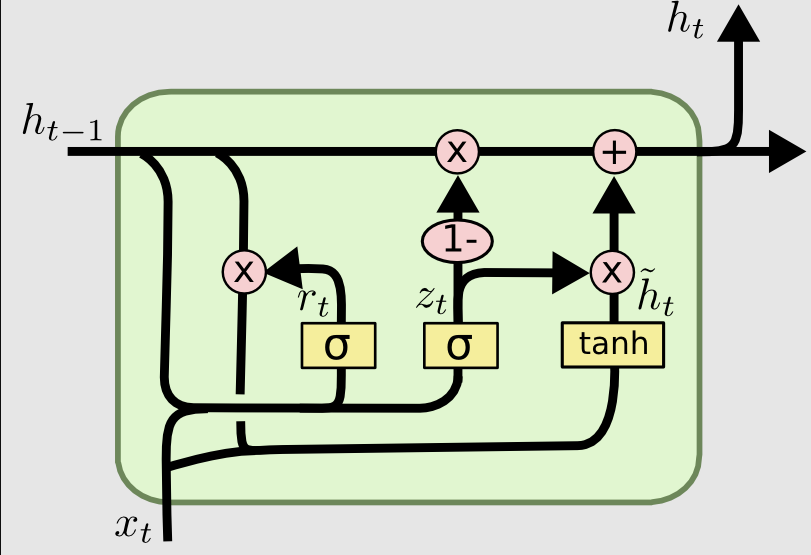
\includegraphics[keepaspectratio=true,height=0.8\paperheight,width=0.9\linewidth]{Images/celda gru.png}
\end{figure}
    
\end{frame}